\newpage
\section{Komunikacja między mikroserwisami}
\label{section:komunikacja-miedzy-serwisami}
\subsection{Broker wiadomości}
Aby mikroserwisy mogły działać poprawnie, potrzebują wymieniać ze sobą informacje 
w sposób szybki i niezawodny. W przypadku komunikacji nie wymagającej żadnej interakcji 
z użytkownikiem, jednym z rozwiązań jest wykorzystanie brokera wiadomości, który pełni 
rolę pośrednika przekazującego wiadomości między mikroserwisami. Do grona takich narzędzi 
należy RabbitMQ. Spośród konkurencyjnych rozwiązań wyróżnia się tym, że jest to 
narzędzie typu open source, ponadto cechuje się małymi wymaganiami sprzętowymi oraz 
łatwością wdrażania w chmurze. 

RabbitMQ wspiera różne protokoły do przekazywania wiadomości, jednak domyślnie 
wykorzystuje protokół AMQP 0-9-1 (ang. \textit{advanced message queuing protocol}). Uogólniony 
schemat, na którym opiera się protokół, został przedstawiony na rysunku \ref{fig:schemat-amqp}.

\begin{figure}[h]
    \centering
    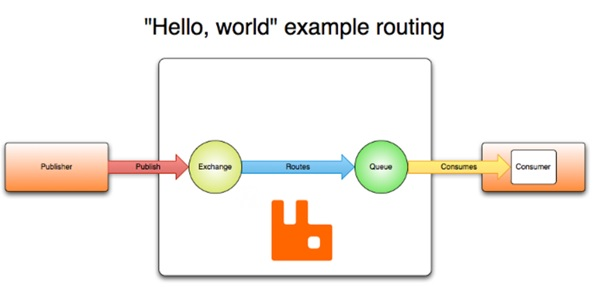
\includegraphics[width=1\textwidth]{amqp_schema.jpg}
    \caption{Schemat protokołu AMQP 0-9-1. Źródło: \cite{rabbitmq2022}}
    \label{fig:schemat-amqp}
\end{figure}

Wydawcy wiadomości (ang. \textit{publisher}) publikują wiadomości do pośrednika, który następnie 
je przekazuje do odpowiednich konsumentów (ang. \textit{consumer}). Ponieważ jest to protokół 
sieciowy, to wydawcy, konsumenci oraz pośrednicy mogą być uruchomieni na różnych 
maszynach. Pośrednik RabbitMQ działa według następujących zasad:

\begin{itemize} % lista nienumerowana
    \item Wiadomości są publikowane na giełdy (ang. exchange)
    \item Giełdy mogą być połączone z wieloma kolejkami (ang. \textit{queue})
    \item Zależnie od zastosowanej polityki kopia wiadomości może być przekazana do 
    każdej powiązanej kolejki lub tylko podzbiorowi kolejek
    \item Kolejka po otrzymaniu wiadomości od giełdy przesyła ją do konsumentów
\end{itemize}

Przesyłanie informacji przez sieć wiąże się z ryzykiem tego, że dane nie zostaną 
dostarczone. Wobec tego protokół zapewnia funkcjonalność zwaną potwierdzeniem 
wiadomości (ang. \textit{message acknowledgements}), która gwarantuje otrzymanie wiadomości 
przez konsumentów. Działa ona w ten sposób, że wiadomość jest usuwana z kolejki tylko 
wtedy, gdy uzyska potwierdzenie jej otrzymania od zainteresowanych mikrousług.

Giełdy po otrzymaniu wiadomości od wydawców mogą ją rozesłać do zera lub większej 
liczby kolejek. Używany algorytm routingu zależy od typu wymiany i reguł nazywanych 
powiązaniami (ang. \textit{bindings}). Pośrednicy korzystający z protokołu AMQP 0-9-1 zapewniają 
cztery typy wymiany:

\begin{itemize} % lista nienumerowana
    \item Wymiana bezpośrednia (ang. \textit{direct exchange}) - dostarcza wiadomości do kolejek 
    na podstawie klucza routingu. Jest idealna do wiadomości typu unicast 
    (chociaż może być także używana do wiadomości typu multicast)
    \item Wymiana do wszystkich (ang. \textit{fanout exchange}) - kieruje komunikaty do wszystkich 
    kolejek, które są z nią powiązane, a klucz routingu jest ignorowany. Jeśli do 
    giełdy dowiązanych jest N kolejek, to po publikacji wiadomości przez wydawcę 
    dotrze ona do wszystkich N kolejek. Jest idealna do rozsyłania wiadomości do 
    wszystkich konsumentów
    \item Wymiana tematyczna (ang. \textit{topic exchange}) - kieruje wiadomości do jednej lub 
    wielu kolejek na podstawie dopasowania klucza routingu oraz wzorca użytego do 
    powiązania kolejki z giełdą. Jest często używana do implementacji różnych odmian 
    wzorca publish/subscribe. Typowo używa się jej dla wiadomości typu multicast. 
    Warto ją rozważyć w przypadku, gdy należy dostarczyć wiadomość do wielu 
    konsumentów, które selektywnie wybierają rodzaj wiadomości, które chcą otrzymywać
    \item Wymiana nagłówków (ang. \textit{headers exchange}) - przeznaczona do routingu na 
    podstawie wielu atrybutów, które łatwiej można wyrazić w postaci nagłówków 
    wiadomości niż klucza routingu, który jest ignorowany. Wiadomość uważana jest za 
    zgodną i rozsyłana dalej, jeśli wartość nagłówka jest równa wartości określonej 
    podczas wiązania
\end{itemize}

AMQP 0-9-1 jest protokołem poziomu aplikacji, który używa protokołu TCP do niezawodnego 
przesyłania wiadomości. Połączenia (ang. \textit{connections}) korzystają z metod 
uwierzytelnienia i mogą być chronione za pomocą protokołu TLS. Ze względu na dodatkowe 
środki zapewniające niezawodność zaleca się, aby połączenia między klientem 
a pośrednikiem były ustanawiane na dłuższy okres czasu. W przypadku gdy klient 
potrzebuje nawiązać wiele połączeń, powinien wykorzystać kanały (ang. 
\textit{channels}), o których można myśleć jak o lekkich połączeniach dzielących jedno 
połączenie TCP. Każda operacja przeprowadzana przez klienta odbywa się z użyciem 
kanału, a komunikacja na różnych kanałach jest od siebie całkowicie odseparowana. 
Z tego względu każda metoda zawiera identyfikator kanału dla rozróżnienia, przez 
który kanał należy wysłać wiadomość.

\subsubsection{MassTransit}

Przy tworzeniu systemu została wykorzystana szyna danych o nazwie MassTransit 
przeznaczona dla aplikacji napisanych w modelu (ang. \textit{framework}) .NET Core
\cite{masstransit2022}. Zapewnia ona poziom 
abstrakcji umożliwiający wykorzystanie wielu różnych pośredników wiadomości, w 
tym RabbitMQ. Spośród wielu swoich zalet, szyna zapewnia:

\begin{itemize} % lista nienumerowana
    \item Równoczesne, asynchroniczne przetwarzanie wiadomości dla zwiększenia 
    przepustowości
    \item Zarządzanie połączeniem. Jeśli dany mikroserwis zostanie rozłączony 
    z pośrednikiem wiadomości, MassTransit spróbuje połączyć się ponownie oraz 
    przywrócić dotychczasowe giełdy, kolejki, a także połączenia między nimi
    \item Serializacja danych. Pośrednik wiadomości RabbitMq przesyła wiadomości 
    w postaci bajtów. Aby za jego pomocą przesłać obiekty specyficzne dla języka 
    C\#, trzeba zapisać je w odpowiednim formacie, w procesie zwanym serializacją. 
    MassTransit implementuje narzędzia do serializacji obiektów
    \item Testy jednostkowe. MassTransit zawiera implementację przygotowaną specjalnie 
    do testów w taki sposób, by testy nie były zależne od reszty infrastruktury 
    systemu. Przykładem jest poniższa metoda:
\end{itemize}

\begin{addmargin}[0mm]{10mm}
\begin{lstlisting}
    internal static async Task 
    PublishAndWaitToBeConsumed<T>(
        T @event, 
        InMemoryTestHarness testHarness)
    {
        var messageIdentifier = 
            await PublishMessage(@event, testHarness);

        var messageHasBeenConsumed = 
        await testHarness
            .Consumed
            .Any(x => 
            x.Context.MessageId == messageIdentifier);
        messageHasBeenConsumed.Should().BeTrue();

        var message = 
        await testHarness!
            .Consumed
            .SelectAsync(x => 
            x.Context.MessageId == messageIdentifier)
            .First();

        message.Exception.Should()
            .BeNull(
                "Message has been consumed 
                without any errors");
    }
    \end{lstlisting}
\end{addmargin}

Metoda publikuje testową wiadomość, po czym sprawdza, czy została prawidłowo 
przetworzona. 

Dzięki zastosowaniu szyny danych tworzenie konsumentów oraz publikowanie wiadomości 
staje się dużo łatwiejsze. Aby utworzyć nowego konsumenta, wystarczy jedynie utworzyć 
nową klasę implementującą interfejs \textit{IConsumer<T>}, gdzie \textit{T} jest oczekiwanym typem 
wiadomości. Klasa musi zawierać implementację metody 
\textit{Consume(ConsumeContext<MeasurementSentEvent> context)}, która zawiera logikę 
przetwarzania wiadomości. Przykładem jest poniższa metoda:

\begin{addmargin}[0mm]{10mm}
\begin{lstlisting}
    public async Task Consume(
        ConsumeContext<MeasurementSentEvent> context)
    {
        var policiesEvaluationResultEvent = 
        await _evaluatePoliciesCommand
            .Handle(context.Message);

        await _eventPublisher
            .Publish(policiesEvaluationResultEvent);
        _logger.LogInformation(
            $"PoliciesEvaluationResultEvent sent 
            from PolicyNode. Message: 
            {policiesEvaluationResultEvent.Message}");
    }

    \end{lstlisting}
\end{addmargin}
    
Zapisuje ona w logach szczegóły dotyczące przychodzącej wiadomości, przetwarza 
otrzymane wartości, po czym publikuje nową wiadomość o innym typie, której konsument 
jest implementowany przez inny mikroserwis.

\subsubsection{Połączenie mikroserwisów z brokerem wiadomości}

Utworzone w ramach pracy mikroserwisy łączą się z brokerem wiadomości i w ten sposób wymieniają między
sobą dane. Mogą one być połączone w różny sposób, zależnie od oczekiwanego rezultatu. Dwa główne
przypadki zostały przedstawione na rysunku \ref{fig:rabbitmq-polaczenie}.

\begin{figure}[h]
    \centering
    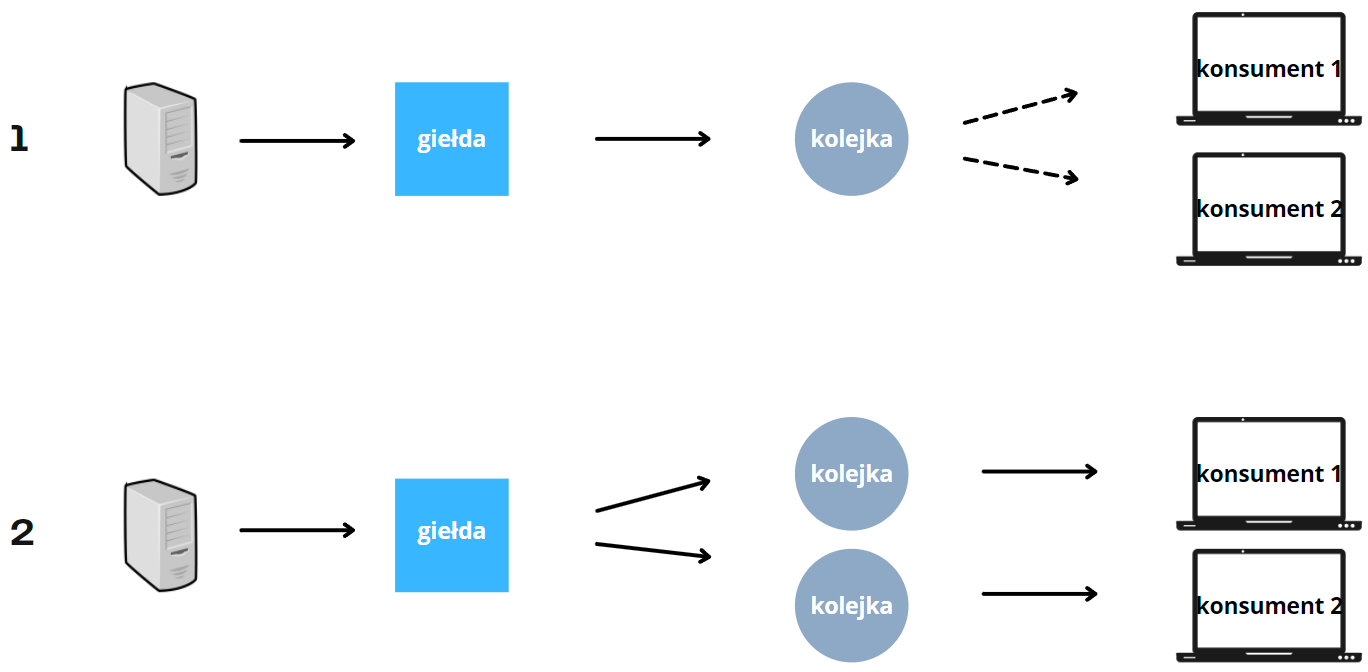
\includegraphics[width=1\textwidth]{rabbitmq_schema.jpg}
    \caption{Rodzaje połączenia z brokerem wiadomości. Opracowanie własne}
    \label{fig:rabbitmq-polaczenie}
\end{figure}

\begin{enumerate}
    \item W pierwszym przypadku celem jest wysłanie wiadomości tylko do jednego konsumenta. Jedną
    z występujących sytuacji jest przetwarzanie otrzymanych z czujników pomiarów przez SSPS. 
    Wykonanie tej samej operacji przez kilka instancji tego serwisu byłoby stratą
    dostępnych zasobów. Aby osiągnąć ten efekt, wszystkie instancje tego serwisu powinny być dołączone 
    do jednej kolejki. Wtedy kolejka wysyła przychodzące pomiary tylko do wybranej przez siebie instancji.
    Wybór odbywa się za pomocą mechanizmu szeregowania procesów Round-robin.
    \item W drugim przypadku celem jest wysłanie wiadomości do wielu konsumentów. Jedną z występujących
    sytuacji jest wysłanie wyniku przetwarzania pomiarów do wszystkich pracowników oraz administratorów
    posiadających uprawnienia do jego wyświetlenia. Aby osiągnąć ten efekt, każda instancja serwisów
    otrzymujących wynik (w tym wypadku są to AAS oraz EAS)
    powinna być dołączona do osobnej kolejki, z których wszystkie dołączone są do tej samej giełdy
    publikującej wiadomości. W ten sposób kopia wysłanej przez wydawcę wiadomości zostanie dostarczona
    do każdej instancji.
\end{enumerate}

\subsection{Styki}

Mikroserwisy mogą komunikować się między sobą przy użyciu oferowanych przez nie 
styków (ang. \textit{Application Programming Interface}). Definiują parametry wymagane 
do realizacji usługi oraz zbiór danych zwracany w odpowiedzi.

Mikrousługi aplikacyjne oraz mikrousługi danych oferują styki zwracające jasno 
zdefiniowany zbiór danych. Zostały one szczegółowo opisane w poniższych podrozdziałach. 
Każda z oferowanych usług zawiera:

\begin{itemize} % lista nienumerowana
    \item Krótki opis funkcjonalności
    \item Wykorzystywany czasownik protokołu http. Jeden z GET, POST, UPDATE, DELETE
    \item wymagane parametry wejściowe
    \item numer statusu oraz typ zwracanego obiektu
\end{itemize}

\subsubsection{Usługi udostępniane przez mikrousługę danych adresów}

\begin{xltabular}{1\textwidth} { 
        | c    
        | c
        | X | }
        \caption{Usługi udostępniane przez ADS} \label{tab:styki-addresses} \\
        \hline
    \textbf{Ścieżka} & 
    \multicolumn{2}{c|}{GET /addresses-api/addresses/\{addressId\}} \\
    \hline
    \textbf{Opis} & 
    \multicolumn{2}{c|}{\makecell{Zwraca informacje na temat adresu o danym identyfikatorze}} \\    \hline
    \textbf{Odpowiedź} &
    \textbf{Kod odpowiedzi} &
    \textbf{Schemat} \\
    \hline
    {} & 200 & AddressDtoJsonApiDocument \\
    \hline
    {} & 404 & JsonApiError \\
    \hline
    \hline
    \hline
    \textbf{Ścieżka} & 
    \multicolumn{2}{c|}{POST /addresses-api/addresses} \\
    \hline
    \textbf{Opis} & 
    \multicolumn{2}{c|}{\makecell{Tworzy nowy adres o parametrach podanych \\ w modelu AddNewAddressCommand}} \\    \hline
    \textbf{Odpowiedź} &
    \textbf{Kod odpowiedzi} &
    \textbf{Schemat} \\
    \hline
    {} & 201 & AddressDtoJsonApiDocument \\
    \hline
    {} & 400 & JsonApiError \\
    \hline
    \hline
    \hline
    \textbf{Ścieżka} & 
    \multicolumn{2}{c|}{GET /addresses-api/cities/\{cityId\}} \\
    \hline
    \textbf{Opis} & 
    \multicolumn{2}{c|}{\makecell{Zwraca informacje na temat miasta o danym identyfikatorze}} \\    \hline
    \textbf{Odpowiedź} &
    \textbf{Kod odpowiedzi} &
    \textbf{Schemat} \\
    \hline
    {} & 200 & CityDtoJsonApiDocument \\
    \hline
    {} & 404 & JsonApiError \\
    \hline
    \hline
    \hline
    \textbf{Ścieżka} & 
    \multicolumn{2}{c|}{GET /addresses-api/countries/\{countryId\}} \\
    \hline
    \textbf{Opis} & 
    \multicolumn{2}{c|}{\makecell{Zwraca informacje na temat kraju o danym identyfikatorze}} \\    \hline
    \textbf{Odpowiedź} &
    \textbf{Kod odpowiedzi} &
    \textbf{Schemat} \\
    \hline
    {} & 200 & CountryDtoJsonApiDocument \\
    \hline
    {} & 404 & JsonApiError \\
    \hline
    \hline
    \hline
    \textbf{Ścieżka} & 
    \multicolumn{2}{c|}{GET /addresses-api/postal-codes/\{postalCodeId\}} \\
    \hline
    \textbf{Opis} & 
    \multicolumn{2}{c|}{\makecell{Zwraca informacje na temat kodu \\pocztowego o danym identyfikatorze}} \\    \hline
    \textbf{Odpowiedź} &
    \textbf{Kod odpowiedzi} &
    \textbf{Schemat} \\
    \hline
    {} & 200 & PostalCodeDtoJsonApiDocument \\
    \hline
    {} & 404 & JsonApiError \\
    \hline
    \end{xltabular}

\subsubsection{Usługi udostępniane przez mikrousługę danych organizacji}


    
\begin{xltabular}{1\textwidth} { 
        | c    
        | c
        | X | }
        \caption{Usługi udostępniane przez FDS} \label{tab:styki-facilities} \\
        \hline
    \textbf{Ścieżka} & 
    \multicolumn{2}{c|}{GET /facilities-api/affiliates/\{affiliateId\}} \\
    \hline
    \textbf{Opis} & 
    \multicolumn{2}{c|}{\makecell{Zwraca informacje na temat oddziału o danym identyfikatorze}} \\    \hline
    \textbf{Odpowiedź} &
    \textbf{Kod odpowiedzi} &
    \textbf{Schemat} \\
    \hline
    {} & 200 & AffiliateDtoJsonApiDocument \\
    \hline
    {} & 404 & JsonApiError \\
    \hline
    \hline
    \hline
    \textbf{Ścieżka} & 
    \multicolumn{2}{c|}{DELETE /facilities-api/affiliates/\{affiliateId\}} \\
    \hline
    \textbf{Opis} & 
    \multicolumn{2}{c|}{\makecell{Usuwa informacje na temat oddziału o danym identyfikatorze}} \\    \hline
    \textbf{Odpowiedź} &
    \textbf{Kod odpowiedzi} &
    \textbf{Schemat} \\
    \hline
    {} & 204 & Brak zawartości \\
    \hline
    {} & 404 & JsonApiError \\
    \hline
    \hline
    \hline
    \textbf{Ścieżka} & 
    \multicolumn{2}{c|}{POST /facilities-api/organizations} \\
    \hline
    \textbf{Opis} & 
    \multicolumn{2}{c|}{\makecell{Tworzy nową organizację o parametrach podanych \\w modelu AddNewOrganizationCommand}} \\    \hline
    \textbf{Odpowiedź} &
    \textbf{Kod odpowiedzi} &
    \textbf{Schemat} \\
    \hline
    {} & 201 & OrganizationDtoJsonApiDocument \\
    \hline
    {} & 400 & JsonApiError \\
    \hline
    {} & 409 & JsonApiError \\
    \hline
    \hline
    \hline
    \textbf{Ścieżka} & 
    \multicolumn{2}{c|}{GET /facilities-api/organizations} \\
    \hline
    \textbf{Opis} & 
    \multicolumn{2}{c|}{\makecell{Zwraca informacje na temat wszystkich organizacji}} \\    \hline
    \textbf{Odpowiedź} &
    \textbf{Kod odpowiedzi} &
    \textbf{Schemat} \\
    \hline
    {} & 200 & OrganizationDtoListJsonApiDocument \\
    \hline
    \hline
    \hline
    \textbf{Ścieżka} & 
    \multicolumn{2}{c|}{GET /facilities-api/organizations/\{organizationId\}} \\
    \hline
    \textbf{Opis} & 
    \multicolumn{2}{c|}{\makecell{Zwraca informacje na temat organizacji o danym identyfikatorze}} \\    \hline
    \textbf{Odpowiedź} &
    \textbf{Kod odpowiedzi} &
    \textbf{Schemat} \\
    \hline
    {} & 200 & OrganizationDtoJsonApiDocument \\
    \hline
    {} & 404 & JsonApiError \\
    \hline
    \hline
    \hline
    \textbf{Ścieżka} & 
    \multicolumn{2}{c|}{DELETE /facilities-api/organizations/\{organizationId\}} \\
    \hline
    \textbf{Opis} & 
    \multicolumn{2}{c|}{\makecell{Usuwa informacje na temat organizacji o danym identyfikatorze}} \\    \hline
    \textbf{Odpowiedź} &
    \textbf{Kod odpowiedzi} &
    \textbf{Schemat} \\
    \hline
    {} & 204 & Brak zawartości \\
    \hline
    {} & 404 & JsonApiError \\
    \hline
    \hline
    \hline
    \textbf{Ścieżka} & 
    \multicolumn{2}{c|}{POST /facilities-api/rooms} \\
    \hline
    \textbf{Opis} & 
    \multicolumn{2}{c|}{\makecell{Tworzy nowe pomieszczenie o parametrach podanych \\w modelu AddNewRoomCommand}} \\    \hline
    \textbf{Odpowiedź} &
    \textbf{Kod odpowiedzi} &
    \textbf{Schemat} \\
    \hline
    {} & 201 & RoomDtoJsonApiDocument \\
    \hline
    {} & 400 & JsonApiError \\
    \hline
    {} & 409 & JsonApiError \\
    \hline
    \hline
    \hline
    \textbf{Ścieżka} & 
    \multicolumn{2}{c|}{GET /facilities-api/rooms/\{roomId\}} \\
    \hline
    \textbf{Opis} & 
    \multicolumn{2}{c|}{\makecell{Zwraca informacje na temat pomieszczenia o danym identyfikatorze}} \\    \hline
    \textbf{Odpowiedź} &
    \textbf{Kod odpowiedzi} &
    \textbf{Schemat} \\
    \hline
    {} & 200 & RoomDtoJsonApiDocument \\
    \hline
    {} & 404 & JsonApiError \\
    \hline
    \hline
    \hline
    \textbf{Ścieżka} & 
    \multicolumn{2}{c|}{DELETE /facilities-api/rooms/\{roomId\}} \\
    \hline
    \textbf{Opis} & 
    \multicolumn{2}{c|}{\makecell{Usuwa informacje na temat pomieszczenia o danym identyfikatorze}} \\    \hline
    \textbf{Odpowiedź} &
    \textbf{Kod odpowiedzi} &
    \textbf{Schemat} \\
    \hline
    {} & 204 & Brak zawartości \\
    \hline
    {} & 404 & JsonApiError \\
    \hline
    \hline
    \hline
    \end{xltabular}

\subsubsection{Usługi udostępniane przez mikrousługę danych reguł}
    
\begin{xltabular}{1\textwidth} { 
        | c    
        | c
        | X | }
        \caption{Usługi udostępniane przez PDS} \label{tab:reguly-styki} \\
        \hline
    \textbf{Ścieżka} & 
    \multicolumn{2}{c|}{POST /policies-api/expected-room-conditions} \\
    \hline
    \textbf{Opis} & 
    \multicolumn{2}{c|}{\makecell{Tworzy nowy zestaw oczekiwanych wartości mierzonych\\parametrów określonych w modelu \\AddNewExpectedRoomConditionsCommand}} \\    \hline
    \textbf{Odpowiedź} &
    \textbf{Kod odpowiedzi} &
    \textbf{Schemat} \\
    \hline
    {} & 201 & OrganizationDtoJsonApiDocument \\
    \hline
    {} & 400 & JsonApiError \\
    \hline
    \hline
    \hline
    \textbf{Ścieżka} & 
    \multicolumn{2}{c|}{\makecell{GET /policies-api/expected-room-\\conditions/\{expectedRoomConditionsId\}}} \\
    \hline
    \textbf{Opis} & 
    \multicolumn{2}{c|}{\makecell{Zwraca informacje na temat zestawu oczekiwanych wartości\\mierzonych parametrów o danym identyfikatorze}} \\    \hline
    \textbf{Odpowiedź} &
    \textbf{Kod odpowiedzi} &
    \textbf{Schemat} \\
    \hline
    {} & 200 & RoomDtoJsonApiDocument \\
    \hline
    {} & 404 & JsonApiError \\
    \hline
    \hline
    \hline
    \textbf{Ścieżka} & 
    \multicolumn{2}{c|}{POST /policies-api/policies} \\
    \hline
    \textbf{Opis} & 
    \multicolumn{2}{c|}{\makecell{Tworzy nową regułę o parametrach określonych \\w modelu AddNewRoomPolicyCommand}} \\    \hline
    \textbf{Odpowiedź} &
    \textbf{Kod odpowiedzi} &
    \textbf{Schemat} \\
    \hline
    {} & 201 & RoomPolicyDtoJsonApiDocument \\
    \hline
    {} & 400 & JsonApiError \\
    \hline
    \hline
    \hline
    \textbf{Ścieżka} & 
    \multicolumn{2}{c|}{POST /policies-api/policies/past-policies} \\
    \hline
    \textbf{Opis} & 
    \multicolumn{2}{c|}{\makecell{Zwraca listę reguł poprzednio obowiązujących \\w pomieszczeniu określonym w modelu GetPastPoliciesCommand}} \\    \hline
    \textbf{Odpowiedź} &
    \textbf{Kod odpowiedzi} &
    \textbf{Schemat} \\
    \hline
    {} & 201 & PastMeasurementsDtoJsonApiDocument \\
    \hline
    {} & 400 & JsonApiError \\
    \hline
    \hline
    \hline
    \textbf{Ścieżka} & 
    \multicolumn{2}{c|}{GET /policies-api/policies/\{roomId\}} \\
    \hline
    \textbf{Opis} & 
    \multicolumn{2}{c|}{\makecell{Zwraca informacje na temat aktualnie obowiązującej \\polityki w pomieszczeniu o danym identyfikatorze}} \\    \hline
    \textbf{Odpowiedź} &
    \textbf{Kod odpowiedzi} &
    \textbf{Schemat} \\
    \hline
    {} & 200 & RoomPolicyDtoJsonApiDocument \\
    \hline
    {} & 404 & JsonApiError \\
    \hline
    \end{xltabular}

\subsubsection{Usługi udostępniane przez mikrousługę danych sensorów}

    
\begin{xltabular}{1\textwidth} { 
        | c    
        | c
        | X | }
        \caption{Usługi udostępniane przez SDS} \label{tab:sensory-styki} \\
        \hline
    \textbf{Ścieżka} & 
    \multicolumn{2}{c|}{GET /sensors-api/sensors} \\
    \hline
    \textbf{Opis} & 
    \multicolumn{2}{c|}{\makecell{Zwraca informacje na temat wszystkich sensorów}} \\    \hline
    \textbf{Odpowiedź} &
    \textbf{Kod odpowiedzi} &
    \textbf{Schemat} \\
    \hline
    {} & 200 & SensorDtoListJsonApiDocument \\
    \hline
    \hline
    \hline
    \textbf{Ścieżka} & 
    \multicolumn{2}{c|}{GET /sensors-api/sensors/room-id/\{roomId\}} \\
    \hline
    \textbf{Opis} & 
    \multicolumn{2}{c|}{\makecell{Zwraca informacje na temat sensorów znajdujących się \\w pomieszczeniu o danym identyfikatorze}} \\    \hline
    \textbf{Odpowiedź} &
    \textbf{Kod odpowiedzi} &
    \textbf{Schemat} \\
    \hline
    {} & 200 & SensorDtoJsonApiDocument \\
    \hline
    {} & 404 & JsonApiError \\
    \hline
    \hline
    \hline
    \textbf{Ścieżka} & 
    \multicolumn{2}{c|}{POST /sensors-api/sensors/sensor-name} \\
    \hline
    \textbf{Opis} & 
    \multicolumn{2}{c|}{\makecell{Zwraca informacje na temat sensorów o parametrach \\określonych w modelu GetSensorBySensorNameCommand}} \\    \hline
    \textbf{Odpowiedź} &
    \textbf{Kod odpowiedzi} &
    \textbf{Schemat} \\
    \hline
    {} & 200 & SensorDtoJsonApiDocument \\
    \hline
    {} & 400 & JsonApiError \\
    \hline
    \hline
    \hline
    \textbf{Ścieżka} & 
    \multicolumn{2}{c|}{GET /sensors-api/sensors/\{sensorId\}} \\
    \hline
    \textbf{Opis} & 
    \multicolumn{2}{c|}{\makecell{Zwraca informacje na temat sensorów o danym identyfikatorze}} \\    \hline
    \textbf{Odpowiedź} &
    \textbf{Kod odpowiedzi} &
    \textbf{Schemat} \\
    \hline
    {} & 200 & SensorDtoJsonApiDocument \\
    \hline
    {} & 404 & JsonApiError \\
    \hline
    \end{xltabular}

\subsubsection{Usługi udostępniane przez mikrousługę aplikacyjną administratorów}

\begin{xltabular}{1\textwidth} { 
        | c    
        | c
        | X | }
        \caption{Usługi udostępniane przez AAS} \label{tab:admin-styki} \\
        \hline
    \textbf{Ścieżka} & 
    \multicolumn{2}{c|}{POST /admin-node/addresses} \\
    \hline
    \textbf{Opis} & 
    \multicolumn{2}{c|}{\makecell{Tworzy nowy adres o parametrach określonych \\w modelu AddNewAddressCommand}} \\    \hline
    \textbf{Odpowiedź} &
    \textbf{Kod odpowiedzi} &
    \textbf{Schemat} \\
    \hline
    {} & 201 & AddressDtoJsonApiDocument \\
    \hline
    {} & 400 & JsonApiError \\
    \hline
    \hline
    \hline
    \textbf{Ścieżka} & 
    \multicolumn{2}{c|}{POST /admin-node/affiliates} \\
    \hline
    \textbf{Opis} & 
    \multicolumn{2}{c|}{\makecell{Tworzy nowy oddział o parametrach określonych \\w modelu AddNewAffiliateCommand}} \\    \hline
    \textbf{Odpowiedź} &
    \textbf{Kod odpowiedzi} &
    \textbf{Schemat} \\
    \hline
    {} & 201 & AffiliateDtoJsonApiDocument \\
    \hline
    {} & 400 & JsonApiError \\
    \hline
    {} & 409 & JsonApiError \\
    \hline
    \hline
    \hline
    \textbf{Ścieżka} & 
    \multicolumn{2}{c|}{GET /admin-node/affiliates} \\
    \hline
    \textbf{Opis} & 
    \multicolumn{2}{c|}{\makecell{Zwraca informacje na temat wszystkich oddziałów}} \\    \hline
    \textbf{Odpowiedź} &
    \textbf{Kod odpowiedzi} &
    \textbf{Schemat} \\
    \hline
    {} & 200 & AdminNodeAffiliateDtoListJsonApiDocument \\
    \hline
    {} & 404 & JsonApiError \\
    \hline
    \hline
    \hline
    \textbf{Ścieżka} & 
    \multicolumn{2}{c|}{GET /admin-node/affiliates/\{affiliateId\}} \\
    \hline
    \textbf{Opis} & 
    \multicolumn{2}{c|}{\makecell{Zwraca informacje na temat oddziału o danym identyfikatorze}} \\    \hline
    \textbf{Odpowiedź} &
    \textbf{Kod odpowiedzi} &
    \textbf{Schemat} \\
    \hline
    {} & 200 & AdminNodeAffiliateDtoJsonApiDocument \\
    \hline
    {} & 404 & JsonApiError \\
    \hline
    \hline
    \hline
    \textbf{Ścieżka} & 
    \multicolumn{2}{c|}{DELETE /admin-node/affiliates/\{affiliateId\}} \\
    \hline
    \textbf{Opis} & 
    \multicolumn{2}{c|}{\makecell{Usuwa informacje na temat oddziału o danym identyfikatorze}} \\    \hline
    \textbf{Odpowiedź} &
    \textbf{Kod odpowiedzi} &
    \textbf{Schemat} \\
    \hline
    {} & 204 & Brak zawartości \\
    \hline
    {} & 404 & JsonApiError \\
    \hline
    \hline
    \hline
    \textbf{Ścieżka} & 
    \multicolumn{2}{c|}{POST /admin-node/organizations} \\
    \hline
    \textbf{Opis} & 
    \multicolumn{2}{c|}{\makecell{Tworzy nową organizację o parametrach określonych \\w modelu AddNewOrganizationCommand}} \\    \hline
    \textbf{Odpowiedź} &
    \textbf{Kod odpowiedzi} &
    \textbf{Schemat} \\
    \hline
    {} & 201 & OrganizationDtoJsonApiDocument \\
    \hline
    {} & 400 & JsonApiError \\
    \hline
    {} & 409 & JsonApiError \\
    \hline
    \hline
    \hline
    \textbf{Ścieżka} & 
    \multicolumn{2}{c|}{GET /admin-node/organizations} \\
    \hline
    \textbf{Opis} & 
    \multicolumn{2}{c|}{\makecell{Zwraca informacje na temat wszystkich organizacji}} \\    \hline
    \textbf{Odpowiedź} &
    \textbf{Kod odpowiedzi} &
    \textbf{Schemat} \\
    \hline
    {} & 200 & \makecell{AdminNodeOrganizationDto\\ListJsonApiDocument} \\
    \hline
    {} & 404 & JsonApiError \\
    \hline
    \hline
    \hline
    \textbf{Ścieżka} & 
    \multicolumn{2}{c|}{GET /admin-node/organizations/\{organizationId\}} \\
    \hline
    \textbf{Opis} & 
    \multicolumn{2}{c|}{\makecell{Zwraca informacje na temat organizacji o danym identyfikatorze}} \\    \hline
    \textbf{Odpowiedź} &
    \textbf{Kod odpowiedzi} &
    \textbf{Schemat} \\
    \hline
    {} & 200 & \makecell{AdminNodeOrganizationDto\\ListJsonApiDocument} \\
    \hline
    {} & 404 & JsonApiError \\
    \hline
    \hline
    \hline
    \textbf{Ścieżka} & 
    \multicolumn{2}{c|}{DELETE /admin-node/organizations/\{organizationId\}} \\
    \hline
    \textbf{Opis} & 
    \multicolumn{2}{c|}{\makecell{Usuwa informacje na temat organizacji o danym identyfikatorze}} \\    \hline
    \textbf{Odpowiedź} &
    \textbf{Kod odpowiedzi} &
    \textbf{Schemat} \\
    \hline
    {} & 204 & Brak zawartości \\
    \hline
    {} & 404 & JsonApiError \\
    \hline
    \hline
    \hline
    \textbf{Ścieżka} & 
    \multicolumn{2}{c|}{POST /admin-node/rooms} \\
    \hline
    \textbf{Opis} & 
    \multicolumn{2}{c|}{\makecell{Tworzy nowe pomieszczenie o parametrach określonych \\w modelu AddNewRoomCommand}} \\    \hline
    \textbf{Odpowiedź} &
    \textbf{Kod odpowiedzi} &
    \textbf{Schemat} \\
    \hline
    {} & 201 & RoomDtoJsonApiDocument \\
    \hline
    {} & 400 & JsonApiError \\
    \hline
    {} & 409 & JsonApiError \\
    \hline
    \hline
    \hline
    \textbf{Ścieżka} & 
    \multicolumn{2}{c|}{POST /admin-node/rooms/get-room} \\
    \hline
    \textbf{Opis} & 
    \multicolumn{2}{c|}{\makecell{Zwraca informacje o pomieszczeniu o parametrach podanych \\w modelu GetRoomCommand}} \\    \hline
    \textbf{Odpowiedź} &
    \textbf{Kod odpowiedzi} &
    \textbf{Schemat} \\
    \hline
    {} & 200 & 	
    AdminNodeRoomDtoJsonApiDocument \\
    \hline
    {} & 404 & JsonApiError \\
    \hline
    \hline
    \hline
    \textbf{Ścieżka} & 
    \multicolumn{2}{c|}{POST /admin-node/rooms/historic-measurements} \\
    \hline
    \textbf{Opis} & 
    \multicolumn{2}{c|}{\makecell{Zwraca informacje o historycznych pomiarach z pomieszczenia \\o parametrach podanych w modelu GetRoomCommand}} \\    \hline
    \textbf{Odpowiedź} &
    \textbf{Kod odpowiedzi} &
    \textbf{Schemat} \\
    \hline
    {} & 200 & 	
    PastMeasurementsDtoJsonApiDocument \\
    \hline
    {} & 400 & JsonApiError \\
    \hline
    \hline
    \hline
    \textbf{Ścieżka} & 
    \multicolumn{2}{c|}{DELETE /admin-node/rooms/\{roomId\}} \\
    \hline
    \textbf{Opis} & 
    \multicolumn{2}{c|}{\makecell{Usuwa informacje na temat pomieszczenia o danym identyfikatorze}} \\    \hline
    \textbf{Odpowiedź} &
    \textbf{Kod odpowiedzi} &
    \textbf{Schemat} \\
    \hline
    {} & 204 & Brak zawartości \\
    \hline
    {} & 404 & JsonApiError \\
    \hline
    \end{xltabular}